\section{Biological Nanopores}

Biological nanopores are small perforations in a lipid bilayer membrane, created
by the central cylindrical cavity of a folded protein assembly. The majority of these
proteins are toxins produced by pathogenic bacteria. Their function in nature is to
perforate the membrane of a cell, causing the cell to depolarize, disrupting vital cell
functions. The perforation also induces an osmotic potential, causing cell nutrients to
spill into the environment. Both effects eventually result in the killing of the
cell.\cite{Peraro2016}

The reason scientists are interested in studying nanopores is related to their size.
These protein structures are generally only a few nanometres in diameter, making them
comparable in size to the tiny transistors found in modern computers. Retrieving
information form nano-scale processes has proven to be a challenging task. Developing
sensors to probe this small length scale is thereby very relevant. This is the exact task
nanopores provide a possible solution to, i.e. spectroscopy at the smallest
scale.

\subsection{Ionic Current Spectroscopy}

In recent years the study of nanopores became a popular research domain, mainly
due to the development of the nanopore-based ionic current spectroscopy. For the case of
biological nanopores, this method is depicted in Figure \ref{fig:IonicCurrentSpec}. A
reservoir, filled with a saline solution, is partitioned into two compartments by a
lipid bilayer. The membrane is perforated using a pore forming protein, for example
$\alpha$-Hemolysin.  When a potential difference is created over the membrane, the
nanopore mediates an ion current between the two liquid-filled compartments.

This ion current through the pore can accurately be measured. If the pore is empty we
refer to the measured current as the open-pore current. However, the applied electric
field also induces forces upon analytes dissolved in the liquid. The net result of these
interactions is a flux of analytes towards and in some cases through the nanopore.
Analytes located inside of the nanopore partially block the flow through the pore,
reducing the measured ion current. The time series of
these current fluctuations can be measured and identified with particular analytes in the
solution. These methods are so precise that they allow for single molecule
spectroscopy.\cite{Howorka2009}

The construction of the molecular machine discussed in this thesis is based on this
spectroscopy technique. Instead of studying analytes in the reservoirs, here
the configuration of a DNA thread trapped inside of the pore can be analysed using the
measured ion current.

It should be noted that besides these biological nanopores there are also inorganic
nanopores in development.\cite{Dekker2007} An example are solid state nanopores created
by making perforations in a semi-conductor wafer. Despite being currently not as
accessible as
biological nanopres, mainly due to their high production costs, this method has some
major advantages.  First of all the material properties provide a chemical robustness not
present in biological nanopores. Secondly, the production process also allows for easy
scalability
and customisability. While currently not as widely used as biological nanopores, solid
state nanopores will prove to be an important asset in the future of nanotechnology.

\begin{figure}[htpb!]
  \centering
  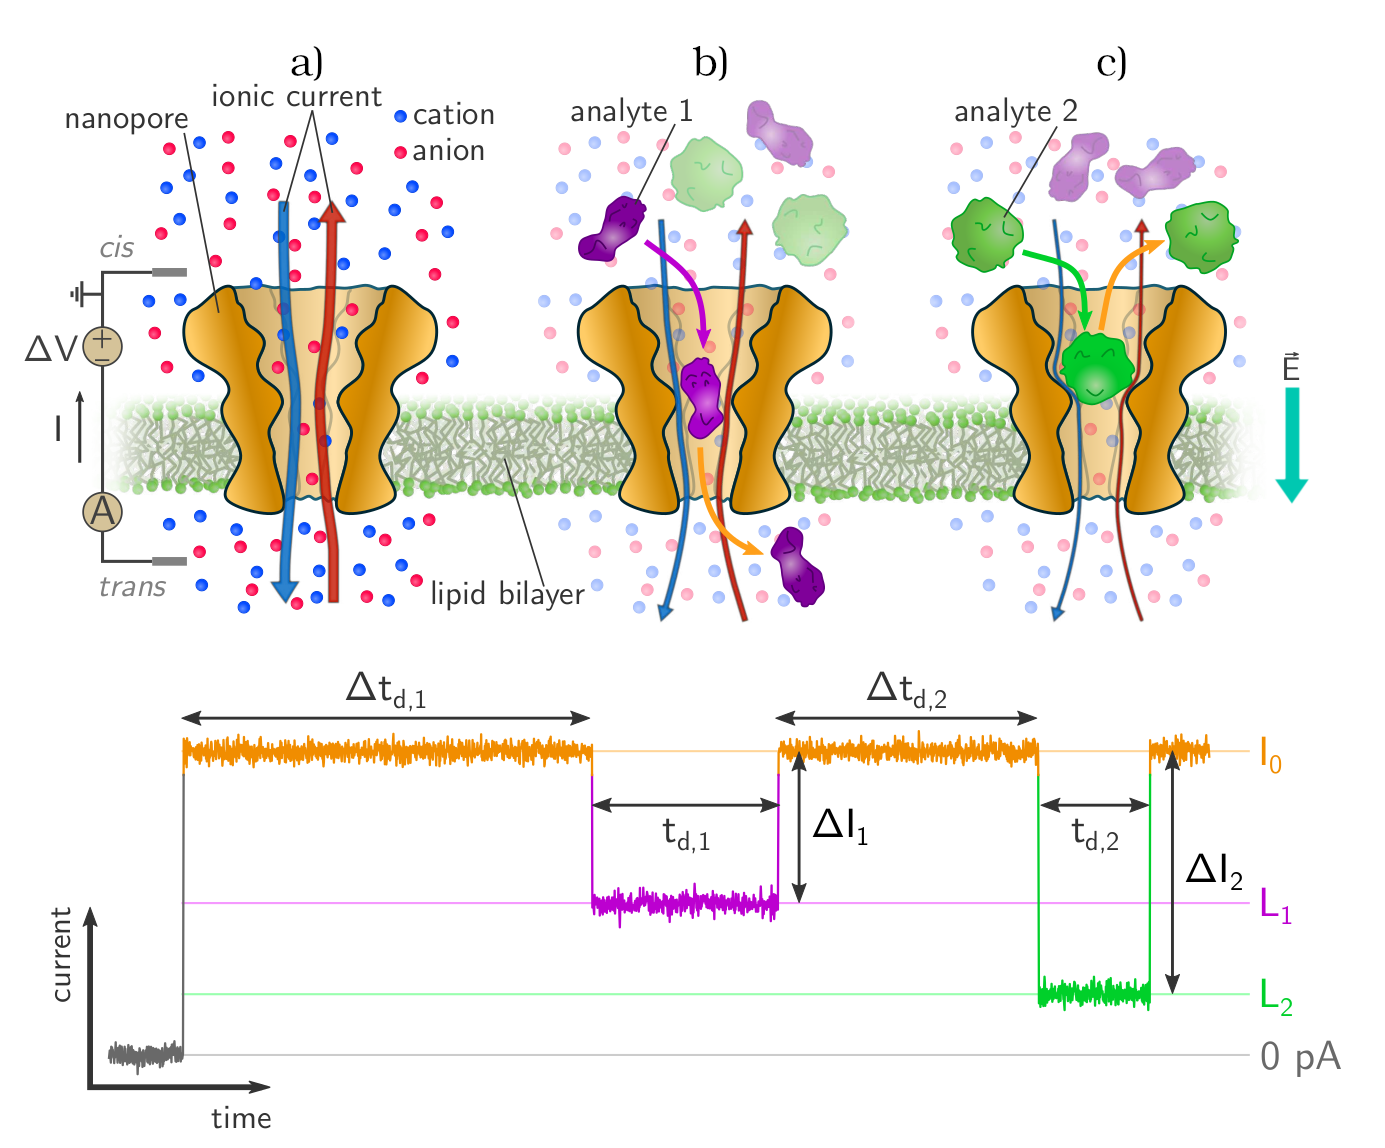
\includegraphics[width=0.72\linewidth, height=7.5cm]{Figures/IonicCurrentSpec2.png}
  \caption[Detailed illustration of ionic current spectroscopy.]{\linespread{0.1}
    {\linespread{0.1}\small  Illustration of the three primary scenarios encountered
      during ionic current
spectroscopy are depicted. Applying a potential difference over the membrane induces a
flow of cations (blue) and anions (red)
through the pore. If the pore is unobstructed, the mediated ion current is referred to
the open-pore current ($I_0$), shown in a). After a certain time $\Delta t_{d,1}$,
analyte $1$ approaches the pore entrance and partially blocks the pore current to the
current level $L_1$, as depicted in b). Due to the size of this analyte it is able to
translocate through the pore with a characteristic dwell time $t_{d,1}$. Both the
duration of translocation and the reduction in ion current depend on the
specific analyte properties . In c) a larger analyte is shown to block the pore current
to a lower level $L_2$. The larger size of this analyte forces it to exit back into the
cis-compartment with a characteristic dwell time $t_{d,2}$. Figure taken from reference
\cite{willems2021}.
}}
  \label{fig:IonicCurrentSpec}
\end{figure}




\subsection{$\alpha$-Hemolysin ($\alpha$-HL)}

The $\alpha$-Hemolysin ($\alpha$-HL) protein is the most commonly used pore forming
protein to create artificial nanopores. It is produced by Staphylococcus aureus, a
bacterium commonly found in the human skin microbiome.\cite{Bhakdi1991}

The $\alpha$-HL pore (PDBID\footnote{An identifier for entries in the Protein Data Bank
(PDB), a database for structural data of large biological
molecules.}:7AHL\cite{Song1859}) is an oligomeric complex
with multiple naturally occurring variations. The most typical configuration
is a heptameric structure, meaning that there are seven subunits, called protomers,
making up the pore complex.
The secondary structure elements consist principally of $\beta$-sheets \footnote{A
secondary protein structure created by hydrogen bonding between parallel or
antiparallel polypeptide strands forming extended $\beta$-pleated sheets.}, making
them a member of the $\beta$-barrel pore-forming toxins. Through both electrostatic and
hydrophobic interactions, the $\alpha$-HL is bound to the membrane of a target cell. Here
the monomers assemble to a 'prepore' complex that transitions to the stable pore complex
by inserting the $\beta$-barrel into the membrane.\cite{SUGAWARA2015226}

Structurally the shape of $\alpha$-HL resembles that of a hollow mushroom, see Figure
\ref{fig:alphaHL}. The total hight of the complex is $11\ nm$ and the maximum width is
measured to be $10\ nm$. The
internal chamber of the pore located at the cis-side of the membrane is called the lumen.
The lumen of $\alpha$-HL is quite constricted having a diameter of merely $3\ nm$.  At
the membrane the lumen chamber transitions into a protein stem, referred to as the
constriction of the pore. Here the diameter of the chamber is reduced to a minimum of
$1.5\ nm$. On the wall of $\alpha$-HL's inside chambers, the charges are relatively
uniformly distributed. \vspace{.4cm}

\begin{figure}[ht!]
  \begin{centering}
  \adjustbox{minipage=1.3em,valign=t}{\subcaption{}\label{sfig:testa}}%
  \begin{subfigure}[t]{\dimexpr.4\linewidth-1.3em\relax}
  \centering
  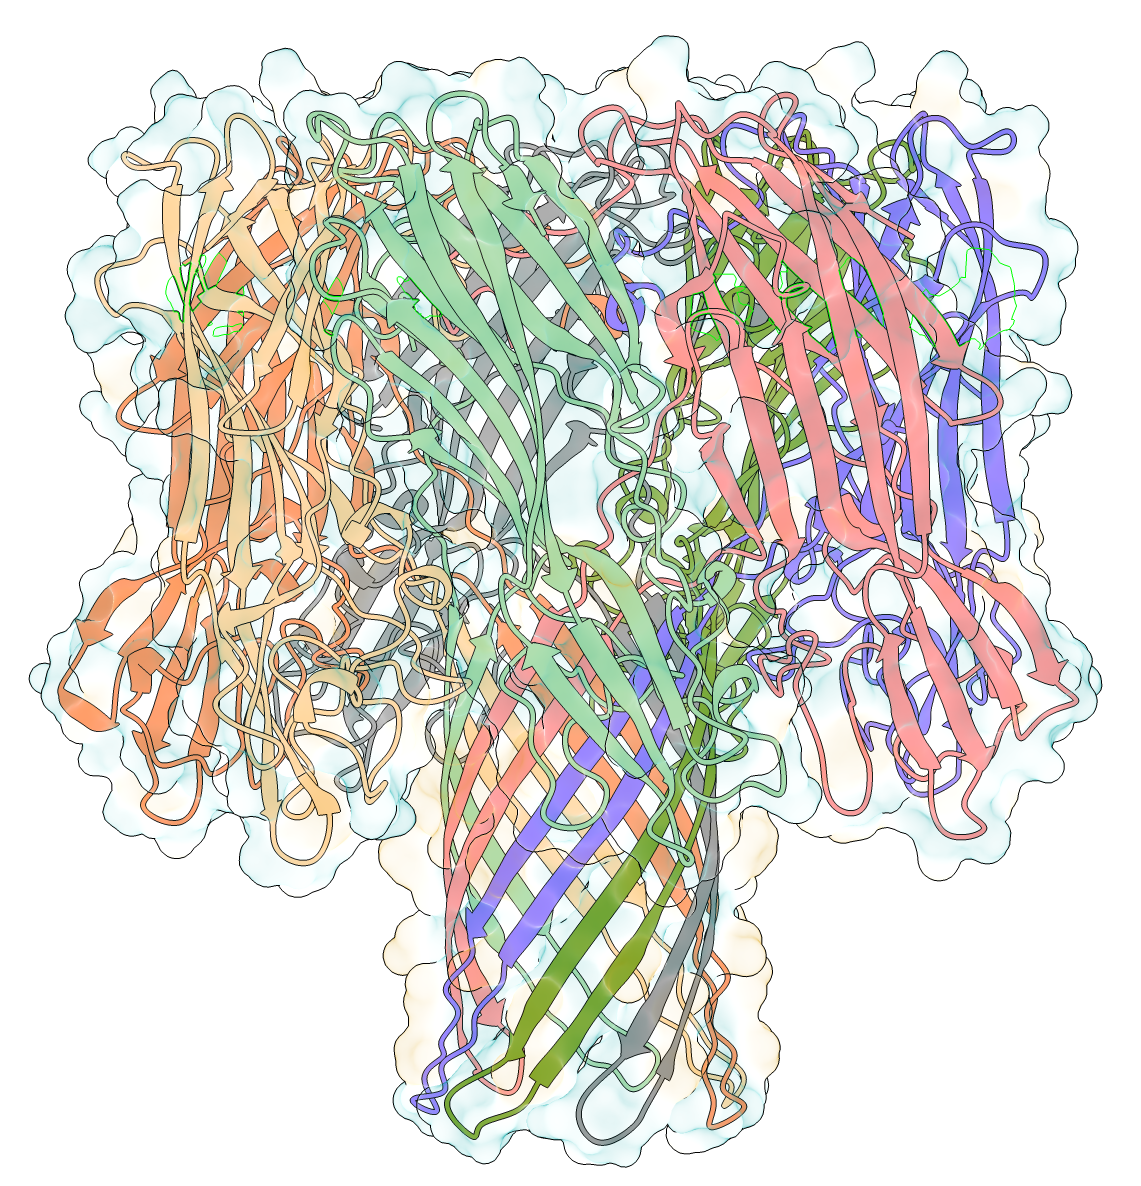
\includegraphics[width=\linewidth,valign=t]{Figures/ahl-front-c.png}
  \end{subfigure}%
  \adjustbox{minipage=1.3em,valign=t}{\subcaption{}\label{sfig:testc}}%
  \begin{subfigure}[t]{\dimexpr.4\linewidth-1.3em\relax}
  \centering
  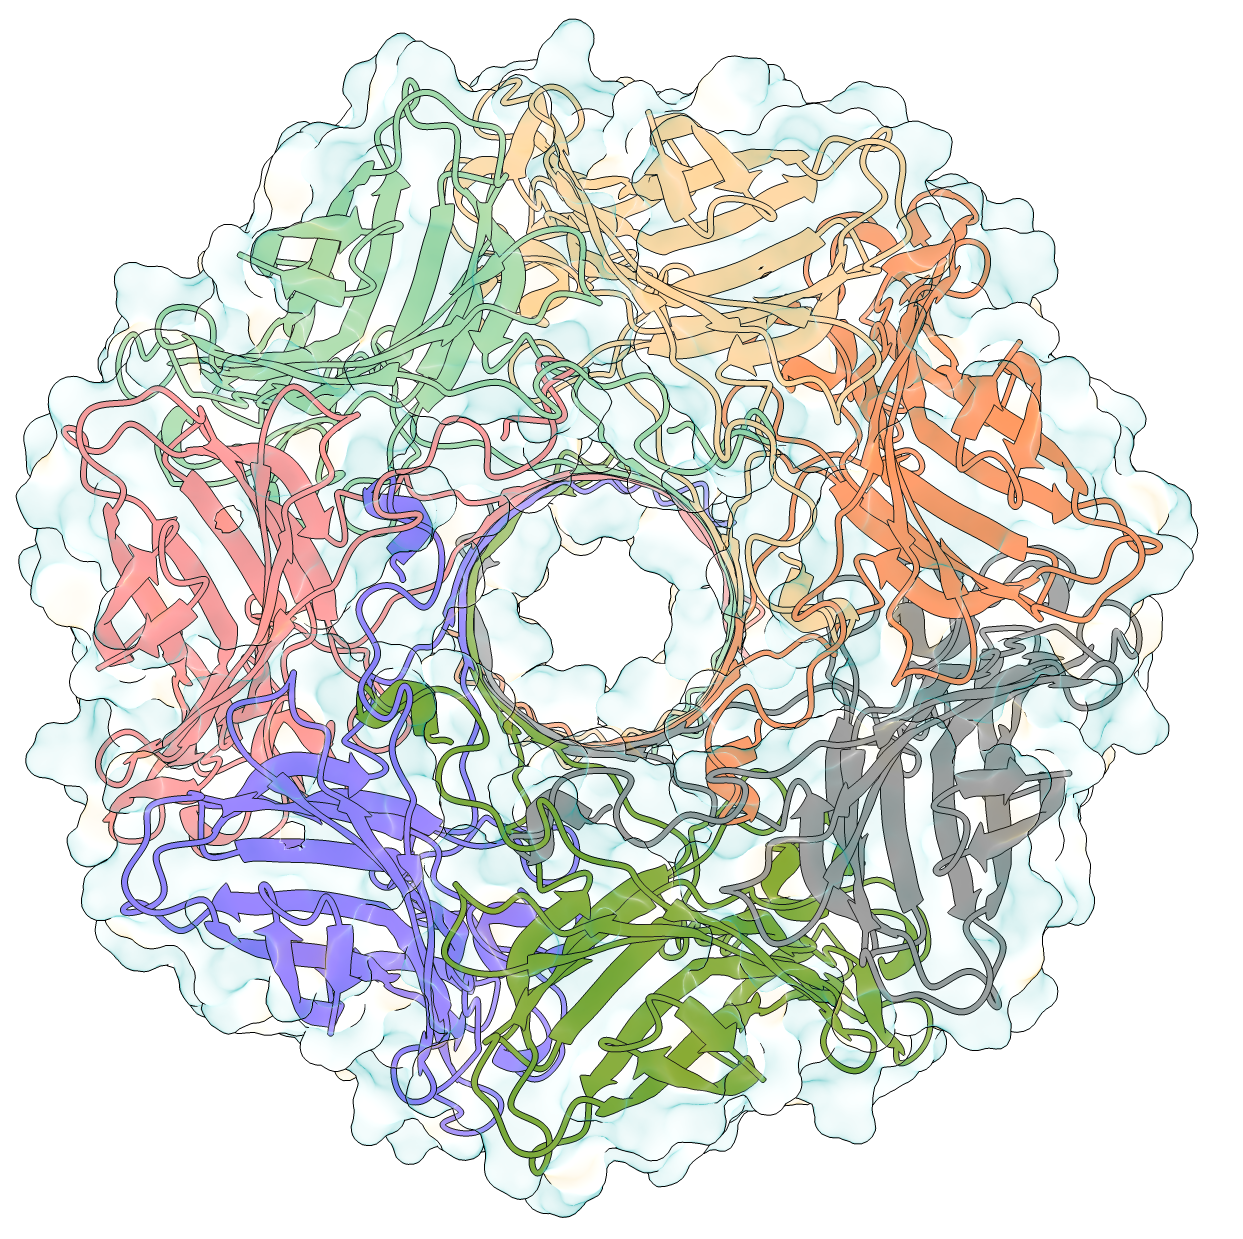
\includegraphics[width=\linewidth,valign=t]{Figures/ahl-top-c.png}
  \end{subfigure}

  \vspace{1.cm}

  \adjustbox{minipage=1.3em,valign=t}{\subcaption{}\label{sfig:testd}}%
  \begin{subfigure}[t]{\dimexpr.4\linewidth-1.3em\relax}
  \centering
  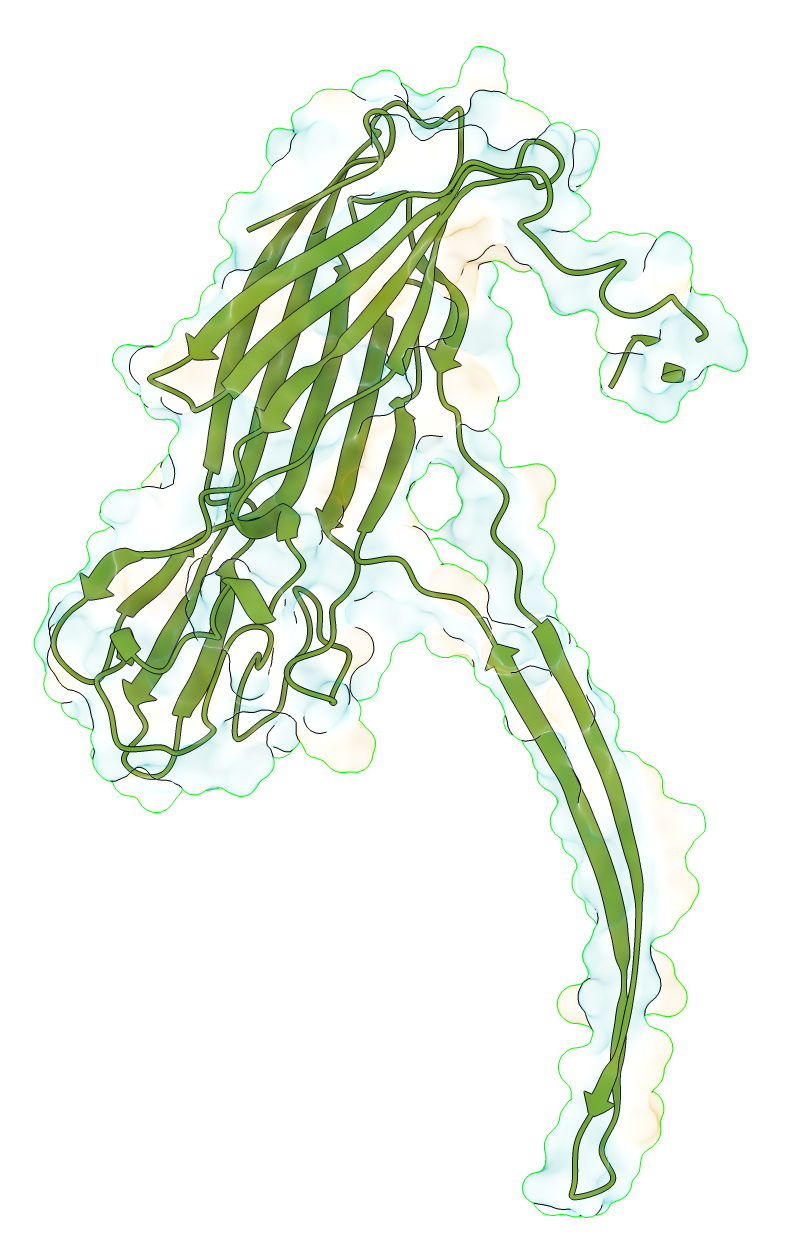
\includegraphics[width=.7\linewidth,valign=t]{Figures/ahl-mon-c.png}
  \end{subfigure}
  \adjustbox{minipage=1.3em,valign=t}{\subcaption{}\label{sfig:testb}}%
  \begin{subfigure}[t]{\dimexpr.4\linewidth-1.3em\relax}
  \centering
  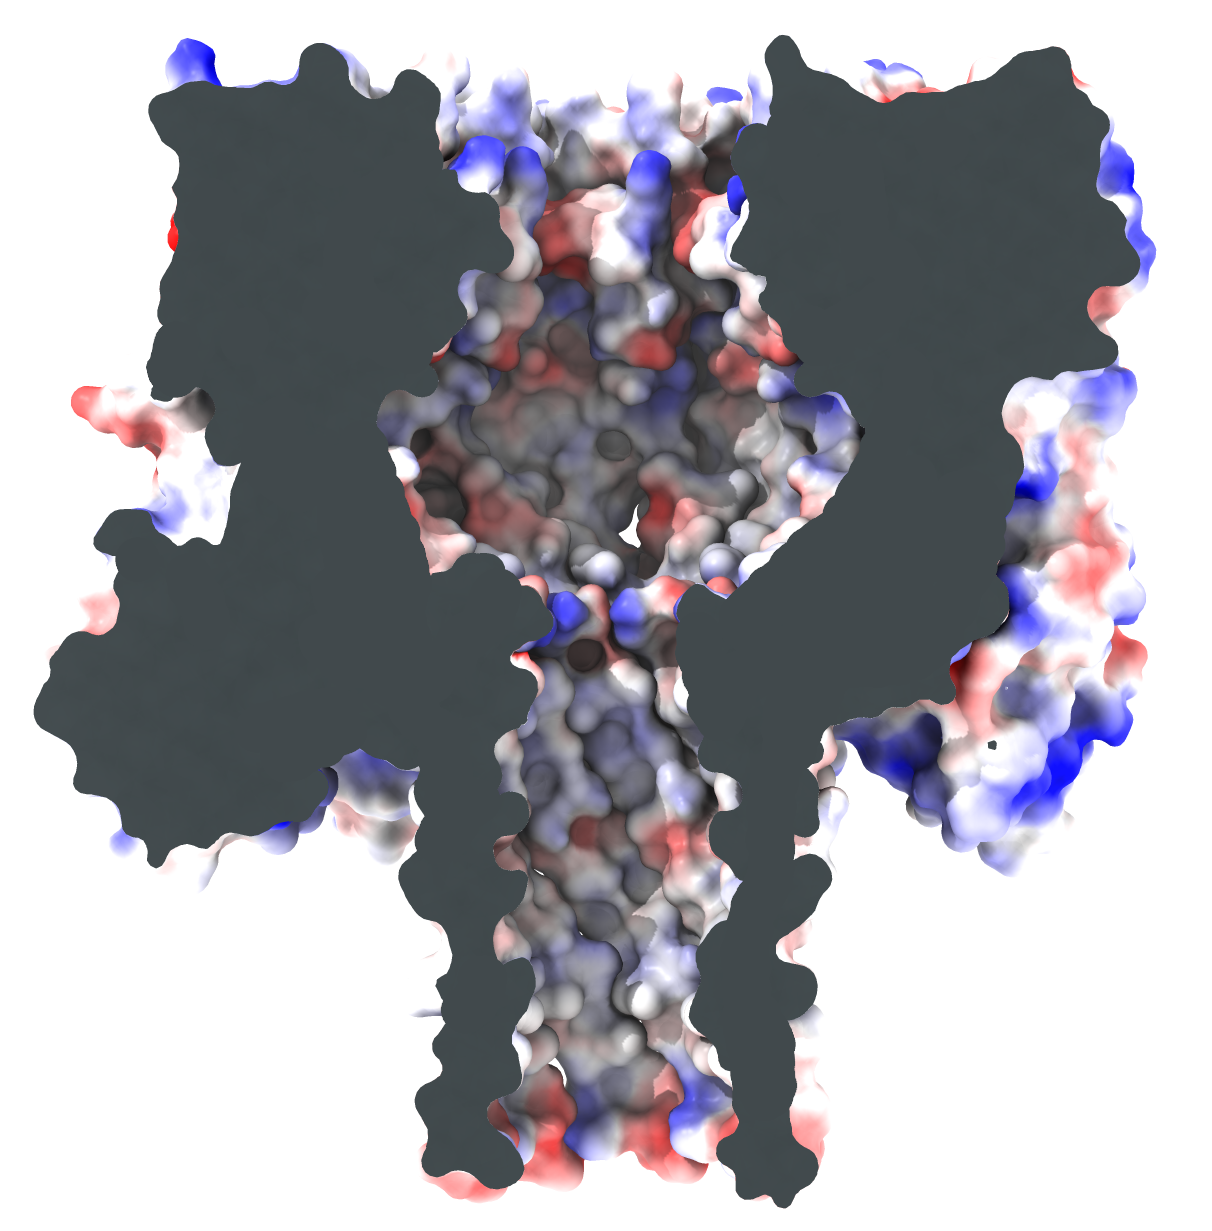
\includegraphics[width=\linewidth,valign=t]{Figures/ahl-elec.png}
  \end{subfigure}%


  \caption[Structural overview of the $\alpha$-Hemolysin ($\alpha$-HL) pore forming
  protein.]{\linespread{0.816}{\small (a) Side view and (b) top view of the
  heptameric $\alpha$-hemolysin ($\alpha$-HL) protein structure. The mushroom shape
  arising from the protomer assembly is clearly shown. (c) Protomer subunit from the
  pore complex, where the two antiparallel $\beta$ strands composing the $\beta$ barrel
  are visible. (d) Estimation of the charge distribution on the cross-section of
  the merged density surface of $\alpha$-HL. All images were rendered using
  ChimeraX. \cite{ChimeraX, Song1859}}}
  \label{fig:alphaHL}

  \end{centering}
\end{figure}

\begin{figure}[ht!]
  \begin{centering}
  \adjustbox{minipage=1.3em,valign=t}{\subcaption{}\label{sfig:testa}}%
  \begin{subfigure}[t]{\dimexpr.3\linewidth-1.3em\relax}
  \centering
  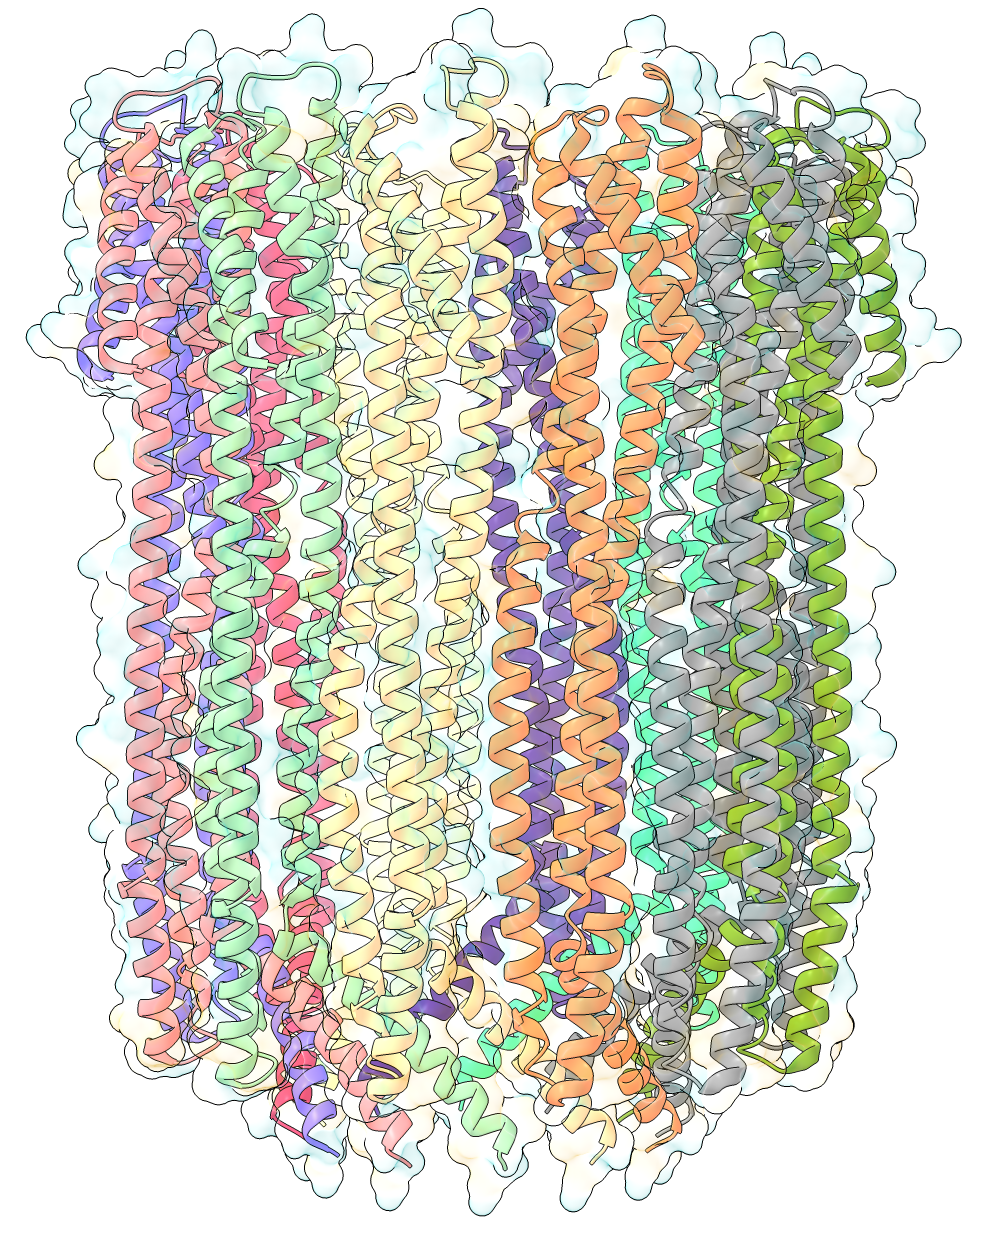
\includegraphics[width=\linewidth,valign=t]{Figures/clya-front-c.png}
  \end{subfigure}%
  \adjustbox{minipage=1.3em,valign=t}{\subcaption{}\label{sfig:testb}}%
  \begin{subfigure}[t]{\dimexpr.35\linewidth-1.3em\relax}
  \centering
  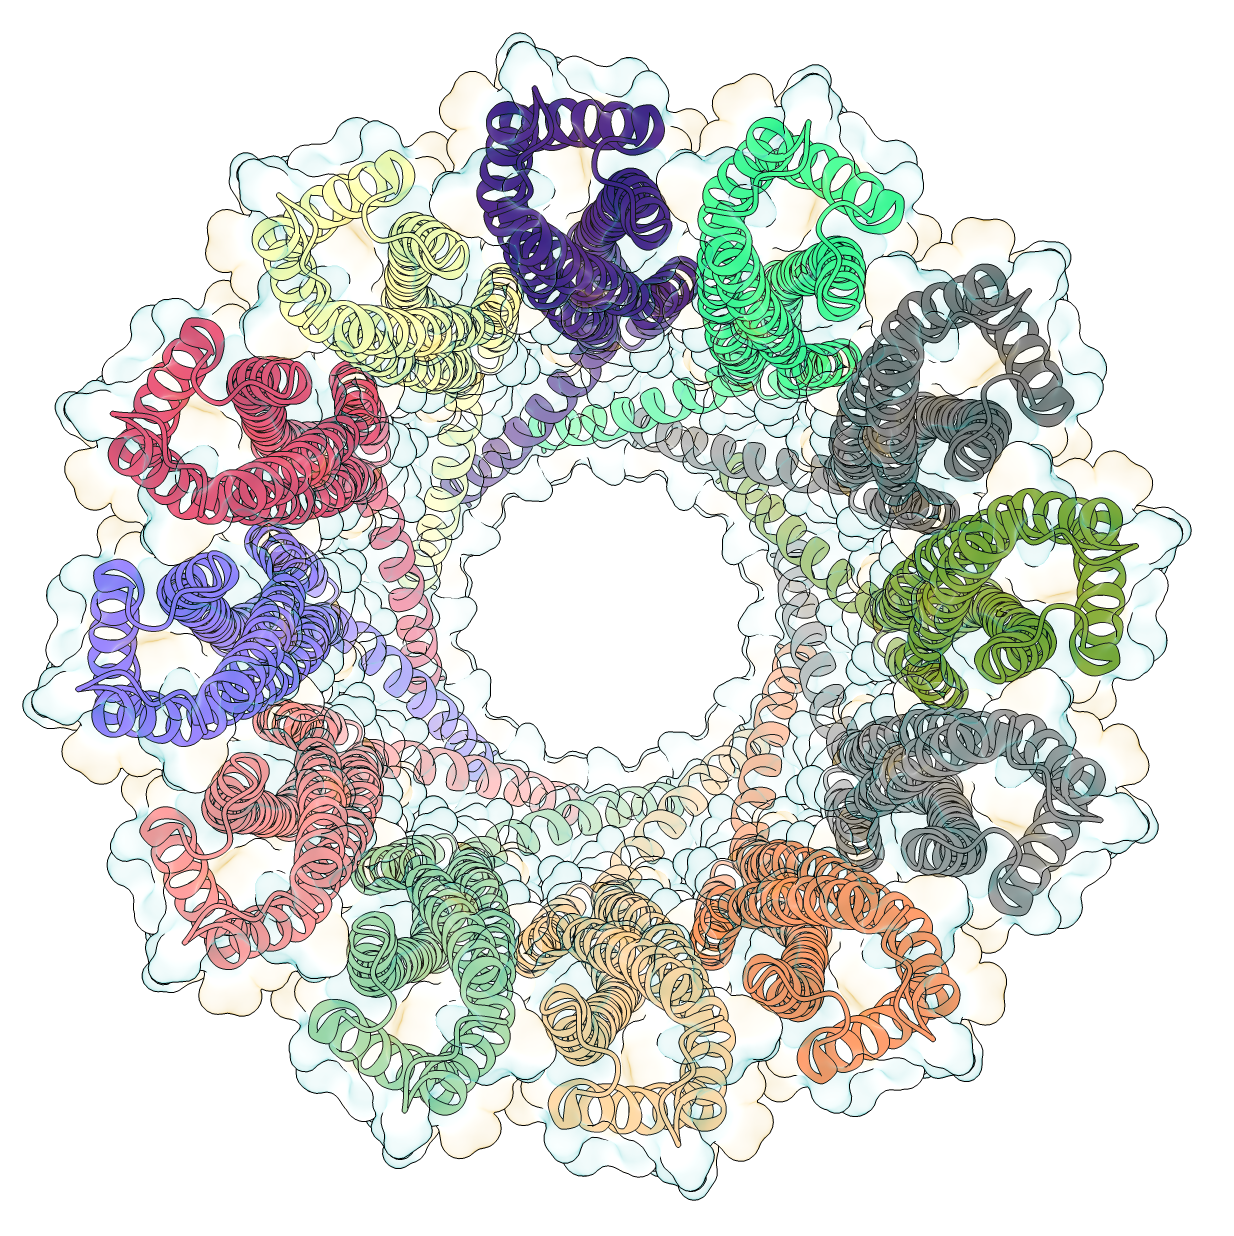
\includegraphics[width=\linewidth,valign=t]{Figures/clya-top-c.png}
  \end{subfigure}

  \vspace{1.cm}

  \adjustbox{minipage=1.3em,valign=t}{\subcaption{}\label{sfig:testb}}%
  \begin{subfigure}[t]{\dimexpr.35\linewidth-1.3em\relax}
  \centering
  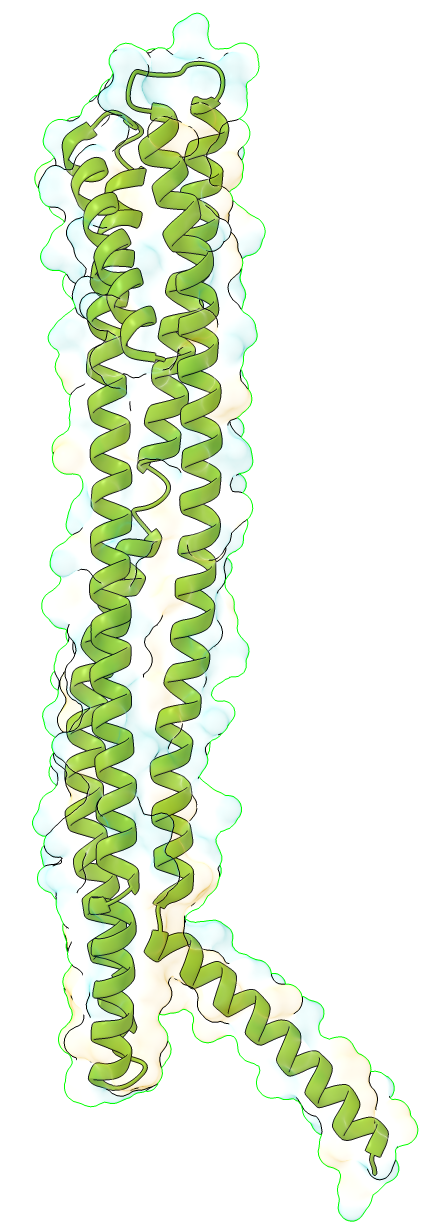
\includegraphics[width=.35\linewidth,valign=t]{Figures/clya-mon-c.png}
  \end{subfigure}%
  \adjustbox{minipage=1.3em,valign=t}{\subcaption{}\label{sfig:testa}}%
  \begin{subfigure}[t]{\dimexpr.3\linewidth-1.3em\relax}
  \centering
  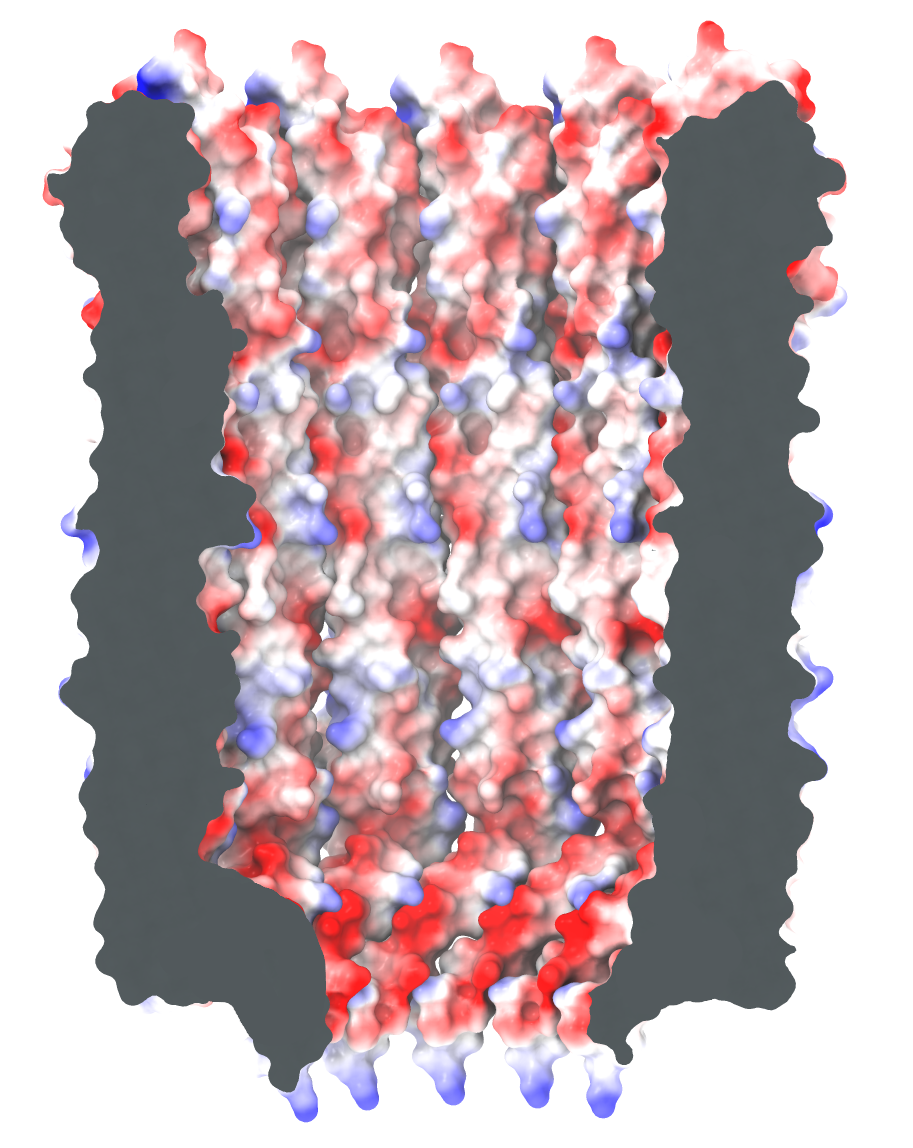
\includegraphics[width=\linewidth,valign=t]{Figures/clya-elec.png}
  \end{subfigure}%

  \caption[Structural overview of the Cytolysin A (ClyA) pore forming
  protein.]{\linespread{0.816}{\small (a) Side view and (b) top view of the
  dodecameric Cytolysin A (ClyA) protein structure. The cylindrical shape
  arising from the protomer assembly is clearly shown. (c) Protomer subunit from the
  pore complex, where the $\alpha$-tongue is visible. (d) Estimation of the charge
  distribution on the cross-section of the merged density surface of ClyA. All images
  were rendered using ChimeraX. \cite{ChimeraX, Peng2019}}}
  \label{fig:ClyA}

  \end{centering}
\end{figure}

\subsection{Cytolysin A (ClyA)}

The Cytolysin A (ClyA) is a larger type of pore forming protein first found to be
secreted by Escherichia coli strains. \cite{Mueller2009} The larger size of its lumen
allows for
different applications compared to smaller complexes like $\alpha$-HL. The
larger diameter of the pore's stem allows for translocation of double stranded DNA, as
demonstrated in the molecular machine discussed in this thesis.

The ClyA pore (PDBID:6MRT\cite{Peng2019}) is an oligomeric complex most typically found
in a dodecameric configuration,  meaning that there are twelve subunits, called
protomers, making up the pore complex. In nature small variations on this configuration
are found.
% \begin{wrapfigure}[38]{l}{0.19\textwidth}
%   \begin{center}
%     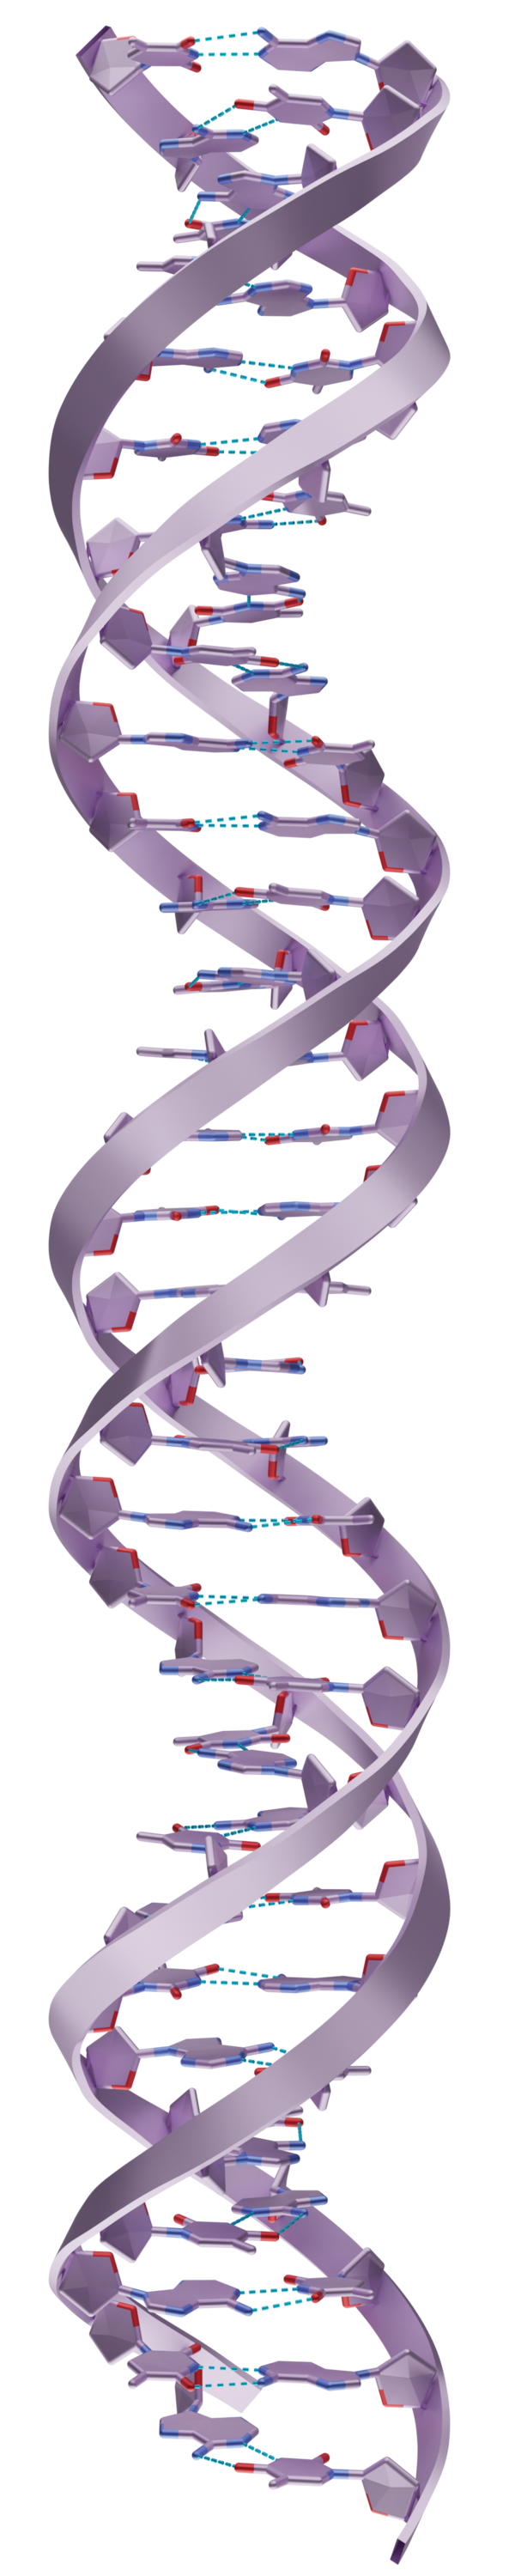
\includegraphics[width=0.2\textwidth]{Figures/DNAStrand.png}
%   \end{center}
%   \caption{\linespread{0.816}{\small An illustration of the double helical structure of
% DNA. Shown is the BDNA form rendered using PDB data and Blender.}}
% \end{wrapfigure}
The secondary structure elements consist principally of
$\alpha$-helices\footnote{A secondary protein structure created by stabilising a coiled
peptide chain with hydrogen bonds, forming a right handed-helix configuration.},
making it a member of the $ \alpha$-pore-forming toxins. The protein formation is induced
by the hydrophobic interactions between the monomers $\beta$-hairpin and the solvent. The
main structural rearrangement in this process consists of swinging out this hairpin and
inserting the resulting $\alpha$-tongue into the membrane. After this transition, the
membrane-bounded monomers oligomerize to form the final pore structure.\cite{Benke2015}

Structurally the shape of ClyA resembles that of two hollow cylinders stacked on top of
each other, see Figure \ref{fig:ClyA}. This cylinder approximation will be important
later on in this thesis, where
it will be used to create a simplified model of the nanopore. The total hight of the
complex is $14\ nm$ and the maximum width is measured to be $11\ nm$. The lumen's size of
this
nanopore differentiates it from the previously discussed $\alpha$-HL. The cis-entrance of
the lumen measures $6\ nm$, while the constricted side of the pore is still $3.6\ nm$ in
diameter.  In contrary to the $\alpha$-HL, the inside surface of ClyA has a net negative
charge, promoting the capturing of positive ions. On the contrary, this excess charge
will induce a significant Coulomb repulsion between the pore and negatively charged
analytes.

